\documentclass[border=2pt]{standalone}
\usepackage{tikz}
\usepackage{graphicx}
\usepackage{capt-of}
\usetikzlibrary{shapes,arrows}

\tikzset{
  treeInode/.style = {align=center, inner sep=1pt, text centered,
    font=\sffamily},
  arn_n/.style = {treeInode, circle, black, draw=black, fill=white, text=black, minimum width=0.5em, minimum height=1em}
    % arbre rouge noir, noeud noir
}
\usetikzlibrary{patterns}

\begin{document}

\tikzset{
  treeInode/.style = {align=center, inner sep=1pt, text centered,
    font=\sffamily},
  arn_n/.style = {treeInode, rectangle, rounded corners=1mm, black, draw=black, fill=black, text=white, font=\sffamily\bfseries, minimum width=1em, minimum height=1em}
    % arbre rouge noir, noeud noir
}
\usetikzlibrary{patterns}

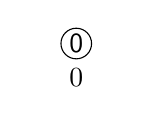
\begin{tikzpicture}[-,>=stealth',level/.style={sibling distance = 0.5cm/#1,
  level distance = 0.6cm}]
\node[arn_n]{0}
; 
\node[below=0.2cm, align=flush center,text width=1cm]{$0$};
\end{tikzpicture}

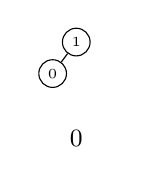
\begin{tikzpicture}[-,>=stealth',level/.style={sibling distance = 0.6cm,
  level distance = 0.4cm}]
\node[arn_n]{\tiny $1$}
  child{
    node[arn_n]{\tiny $0$}
  }
  child[missing]{
  }
; 
\node[below=1cm, align=flush center,text width=1cm]{\small $0$};
\end{tikzpicture}
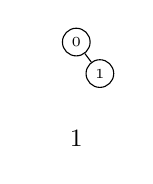
\begin{tikzpicture}[-,>=stealth',level/.style={sibling distance = 0.6cm,
  level distance = 0.4cm}]
\node[arn_n]{\tiny $0$}
	child[missing]{
	}
	child{
		node[arn_n]{\tiny $1$}
	}
; 
\node[below=1cm, align=flush center,text width=1cm]{\small $1$};
\end{tikzpicture}

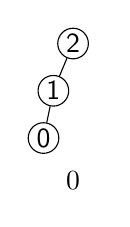
\begin{tikzpicture}[-,>=stealth',level/.style={sibling distance = 0.5cm/#1,
  level distance = 0.6cm}] 
\node[arn_n]{2}
  child{
    node[arn_n]{1}
    child{
      node[arn_n]{0}
    }
    child[missing]{
    }
  }
  child[missing]{
  }
; 
\node[below=1.5cm, align=flush center,text width=0.5cm]{$0$};
\end{tikzpicture}
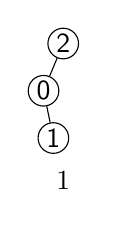
\begin{tikzpicture}[-,>=stealth',level/.style={sibling distance = 0.5cm/#1,
  level distance = 0.6cm}] 
\node[arn_n]{2}
  child{
    node[arn_n]{0}
    child[missing]{
    }
    child{
      node[arn_n]{1}
    }
  }
  child[missing]{
  }
; 
\node[below=1.5cm, align=flush center,text width=0.5cm]{$1$};
\end{tikzpicture}
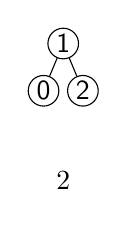
\begin{tikzpicture}[-,>=stealth',level/.style={sibling distance = 0.5cm/#1,
  level distance = 0.6cm}] 
\node[arn_n]{1}
  child{
    node[arn_n]{0}
  }
  child{
    node[arn_n]{2}
  }
; 
\node[below=1.5cm, align=flush center,text width=0.5cm]{$2$};
\end{tikzpicture}
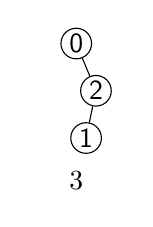
\begin{tikzpicture}[-,>=stealth',level/.style={sibling distance = 0.5cm/#1,
  level distance = 0.6cm}] 
\node[arn_n]{0}
  child[missing]{
  }
  child{
    node[arn_n]{2}
    child{
      node[arn_n]{1}
    }
    child[missing]{
    }
  }
; 
\node[below=1.5cm, align=flush center,text width=1cm]{$3$};
\end{tikzpicture}
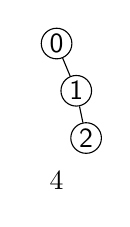
\begin{tikzpicture}[-,>=stealth',level/.style={sibling distance = 0.5cm/#1,
  level distance = 0.6cm}] 
\node[arn_n]{0}
  child[missing]{
  }
  child{
    node[arn_n]{1}
    child[missing]{
    }
    child{
      node[arn_n]{2}
    }
  }
; 
\node[below=1.5cm, align=flush center,text width=0.5cm]{$4$};
\end{tikzpicture}

\end{document}